\documentclass{article}
\usepackage[utf8]{inputenc}
\usepackage{amsmath}
\usepackage{hyperref}
\usepackage{listings}
\usepackage{xcolor}
\usepackage{graphicx}
\usepackage{float}
\usepackage[a4paper, margin=1cm]{geometry}

\lstdefinestyle{python}{
language=Python,
basicstyle=\ttfamily\small,
keywordstyle=\color{blue}\bfseries,
stringstyle=\color{red},
commentstyle=\color{green!50!black},
showstringspaces=false,
breaklines=true
}

\title{Simulación de Eventos Discretos}
\author{Nombre: Darío Hernández Cubilla \\ Grupo: C-311 \\ Telegram: @dhc77}
\date{\today}

\begin{document}

\maketitle


\section{Introducción}
\subsection{Descripción del Proyecto}
Este es un proyecto de simulación de eventos discretos, cuyo objetivo es demostrar conocimientos adquiridos en clases en dicho campo. Se define un modelo de simulación y se realizan experimentos sobre él.
\subsection{Sistema a Simular y Variables de Interés}
Se simulará un sistema con una cola y n servidores en paralelo que atienden clientes de esta, donde se analizará el tiempo de espera promedio de los clientes en un tiempo dado, se llamará un ''día'' SPG. La implementación es generalizable a cualquier número de servidores, con distribuciones posiblemente diferentes. La distribución de llegada también es parametrizable. El único requerimiento es que estas no tengan memoria, ni dependan del tiempo, aunque el sistema es lo suficientemente extensible para que implementar estas funcionalidades sea relativamente sencillo, no era parte del alcance del proyecto.

\section{Detalles de Implementación}
\subsection{Pasos Seguidos para la Implementación}
La implementación es similar a las discutidas en clase, con la diferencia de la parametrizabilidad de la cantidad y el comportamiento de los servidores, también se aceptan ''generadores de prioridad'' para estos, esto es para el caso en que un cliente vea varios servidores libres, se generarán dichas prioridades (que pueden ser constantes), y el cliente elegirá el que tenga un valor mínimo de dicha prioridad.

Se define la clase \texttt{NServerQueue}, que se encuentra en \texttt{m\_g\_k.py}, que es la encargada de manejar la simulación. Esta clase tiene un constructor que recibe una lista de servidores, una función generadora de llegadas y un tiempo final. La función generadora de llegadas es una función que devuelve un número real positivo, que representa el tiempo entre llegadas.

\begin{lstlisting}[style=python, caption={Constructor de clase NServerQueue}]
class NServerQueue:
    def __init__(self, servers: list[Server], arrival_generator: Callable[[], float], end_time: float):
        # ...
\end{lstlisting}

Cada servidor es un objeto que tiene un generador de tiempos de servicio y un generador de prioridades. El generador de tiempos de servicio es una función que devuelve un número real positivo, que representa el tiempo que tarda el servidor en atender a un cliente. El generador de prioridades es una función que devuelve un número entero positivo, que representa la prioridad del servidor cuando hay varios a elegir por un cliente.

\begin{lstlisting}[style=python, caption={Clase Server}]
class Server:
    def __init__(self, service_time_generator: Callable[[], float], priority_generator: Callable[[], int]):
        self.service_time_generator = service_time_generator
        self.priority_generator = priority_generator
\end{lstlisting}

\begin{lstlisting}[style=python, caption={Ejemplo de diferentes combinaciones de servidores}]
import numpy.random as rng

model_1 = NServerQueue(
    servers=[
        Server(lambda: rng.exponential(1/10), lambda: 1),
        Server(lambda: rng.exponential(1/10), lambda: 2),
        Server(lambda: rng.exponential(1/10), lambda: 3),
    ],
    arrival_generator=lambda: rng.exponential(1/20),
    end_time=100
)

model_2 = NServerQueue(
    servers=[
        Server(lambda: rng.exponential(1/20), lambda: 1),
    ],
    arrival_generator=lambda: rng.exponential(1/20),
    end_time=100
)
\end{lstlisting}

El núcleo de la simulación es un ciclo que maneja eventos. Solo hay dos tipos de eventos: llegada (cuando un cliente llega al sistema y se encola o entra al servicio de un servidor si encuentra uno libre), y salida (cuando un cliente termina de ser atendido por un servidor y se va del sistema). Cuando el tiempo actual es mayor que el final se dejan de generar llegadas, y se espera a que todos los clientes en el sistema terminen de ser atendidos. Los eventos se mantienen en una cola con prioridad, donde el próximo evento a procesar se mantiene al tope de la cola.

Además de esto, se guardan ''Snapshots'' de la simulación en cada evento, para inspección más granular de la simulación, esto no es necesario para la aplicación de este proyecto, pero es útil para depuración y análisis posterior. Estos snapshots son objetos que contienen el estado de la simulación en un momento dado.

\begin{lstlisting}[style=python, caption={Clase Snapshot}]
class Snapshot:
    def __init__(self, time: float, people_in_queue: int, people_serviced: list[int], free_servers: set[int], servers_serving: set[int]):
        self.time = time
        self.people_in_queue = people_in_queue # Cantidad de personas en la cola
        self.people_serviced = people_serviced # Cantidad de personas atendidas por cada servidor
        self.free_servers = free_servers # Conjunto de servidores libres
        self.servers_serving = servers_serving # Conjunto de servidores atendiendo
\end{lstlisting}

Finalmente, esta implementación se usa en una notebook de Jupyter, localizada en \texttt{project.ipynb}, donde se pueden ver los resultados obtenidos.

\section{Resultados y Experimentos}
\subsection{Hallazgos de la Simulación}
La posibilidad de parametrizar la cantidad y el comportamiento de los servidores con facilidad sugirió probar diferentes combinaciones de configuraciones, para ver cuáles eran las mejores.

Para esto habría que definir ''mejor'' en este contexto. Simplemente se usó el criterio de minimizar la cantidad promedio de tiempo que un cliente tarda en el sistema en un día dado.

Una pregunta que surge podría ser, es mejor n servidores que despachen clientes a una cierta velocidad, o un servidor que despache a n veces dicha velocidad, siquiera es diferente? Este tipo de pregunta puede ser interesante en muchos contextos, mejorar el servicio existente puede ser más o menos caro que simplemente duplicarlo, y poder demostrar o refutar que estos cambios son equivalentes puede ser valioso por este aspecto.

Como control, se creó una prueba con el mismo modelo comparado contra sí mismo:

\begin{lstlisting}[style=python, caption={Modelo de control}]
# esta es una clase ayudante para encapsular las configuraciones de los modelos
class ModelConfig:
    def __init__(self, servers, arrival_generator, label):
        self.servers = servers
        self.arrival_generator = arrival_generator
        self.label = label

model_config_1 = ModelConfig(
    servers=[
        Server(lambda: rng.exponential(1/2), lambda: 1),
        Server(lambda: rng.exponential(1/2), lambda: 2),
        Server(lambda: rng.exponential(1/2), lambda: 3),
    ],
    arrival_generator=lambda: rng.exponential(1/6),
    label="Model 1: 3 servers, arrival rate 6"
)
\end{lstlisting}


\begin{figure}[H]
   \centering
   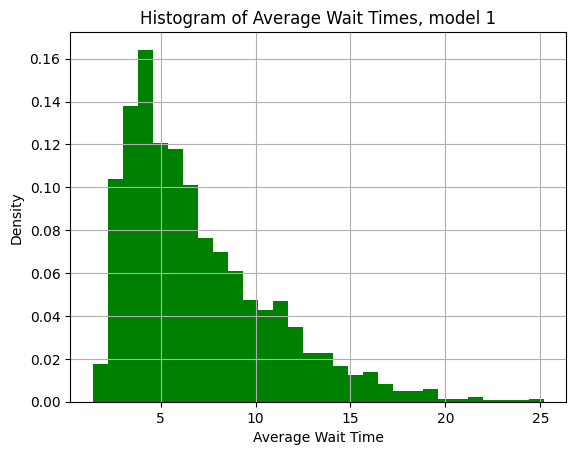
\includegraphics[width=0.8\textwidth]{images/distro_1_1.png}
    \caption{Distribución de tiempos de espera promedio en el sistema para el modelo 1, la primera vez que se simuló}
\end{figure}

\begin{figure}[H]
   \centering
   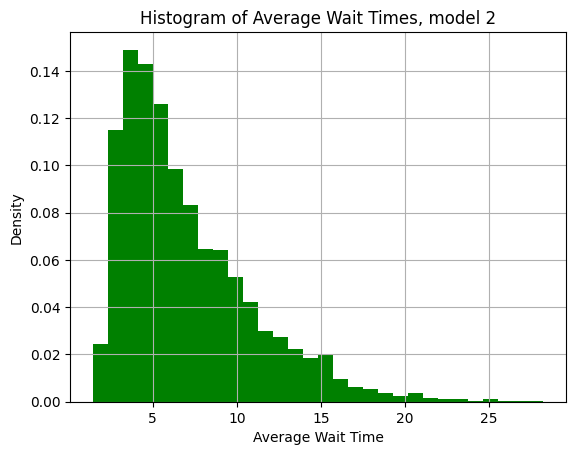
\includegraphics[width=0.8\textwidth]{images/distro_1_2.png}
    \caption{Distribución de tiempos de espera promedio en el sistema para el modelo 1, la segunda vez que se simuló}
\end{figure}

Y finalmente, se comparó el modelo 1 contra un modelo distinto, con un solo servidor, pero con una velocidad de atención del triple y la misma distribución de llegadas: 

\begin{lstlisting}[style=python, caption={Modelo 2}]
model_config_1 = ModelConfig(
    servers=[
        Server(lambda: rng.exponential(1/2), lambda: 1),
        Server(lambda: rng.exponential(1/2), lambda: 2),
        Server(lambda: rng.exponential(1/2), lambda: 3),
    ],
    arrival_generator=lambda: rng.exponential(1/6),
    label="Model 1: 3 servers, arrival rate 6"
)
model_config_2 = ModelConfig(
    servers=[
        Server(lambda: rng.exponential(1/6), lambda: 1),
    ],
    arrival_generator=lambda: rng.exponential(1/6),
    label="Model 1: 1 server, arrival rate 6"
)
\end{lstlisting}

\begin{figure}[H]
   \centering
   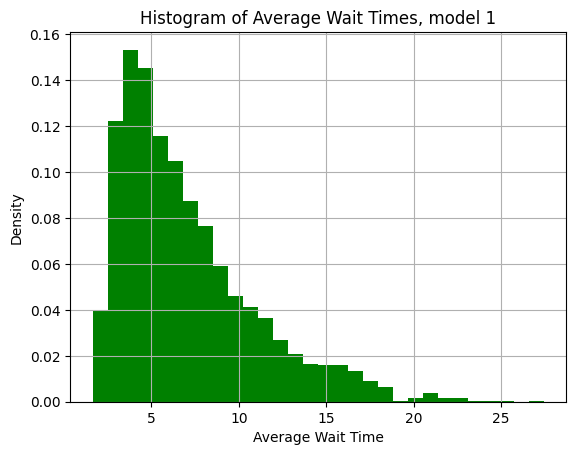
\includegraphics[width=0.8\textwidth]{images/distro_1_3.png}
    \caption{Distribución de tiempos de espera promedio en el sistema para el modelo 2, la primera vez que se simuló}
\end{figure}

\begin{figure}[H]
   \centering
   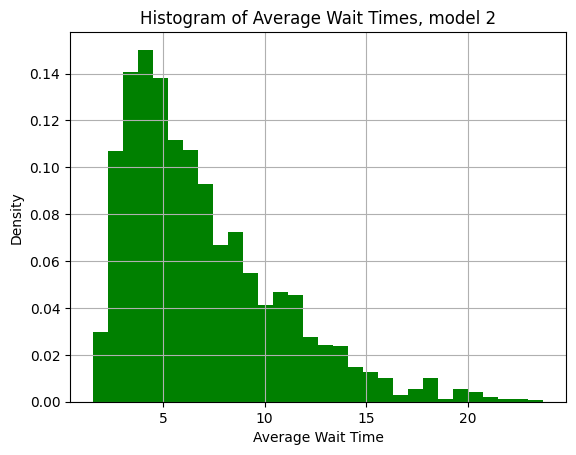
\includegraphics[width=0.8\textwidth]{images/distro_2_1.png}
    \caption{Distribución de tiempos de espera promedio en el sistema para el modelo 2, la segunda vez que se simuló}
\end{figure}

Aparentemente, no existían diferencias notables entre los modelos, pero se debe demostrar esta afirmación con tests de hipótesis.

\subsection{Hipótesis y Validación}

Como se buscaba calcular el valor esperado de la media de la cantidad de tiempo que un cliente pasa en el sistema en un día dado (durante un mismo día, si vemos el tiempo que se demora cada cliente en el sistema como variables aleatorias, no son ni independientes ni idénticamente distribuidas, sin embargo, si analizamos la media de estas variables en un mismo día, obteniendo una nueva variable aleatoria, esta sí es independiente e idénticamente distribuida con las correspondientes a los otros días), se definió un tamaño del intervalo de confianza de 95\% y un error de 0.33 (20 segundos) y se usó como criterio de parada, para dejar de correr simulaciones, cuando $2 \cdot Z_{0.025}\frac{S}{\sqrt{n}} \leq 0.33$, donde S es la desviación estándar de la muestra y n es el tamaño de la muestra.

Para la primera prueba, se creó una prueba de hipótesis de diferencia de medias:

\begin{math}
    \begin{aligned}
    H_0: \overline{X}_1 = \overline{X}_2 \\
    H_1: \overline{X}_1 \neq \overline{X}_2
    \end{aligned}
\end{math}


Donde $\overline{X}_1$ y $\overline{X}_2$ son las medias de los tiempos de espera promedio en el sistema para el modelo 1, la primera y segunda vez que se simuló respectivamente.

Se usó una prueba con la distribución normal (se generaron muchas más de 30 simulaciones) de dos colas (el estadístico utilizado fue $z = \frac{\overline{X}_1 - \overline{X}_2}{\sqrt{\frac{S_1}{n_1} + \frac{S_2}{n_2}}}$), con un nivel de significancia de 0.05, como se esperaba, no se encontraron diferencias marcadas entre las medias.

\begin{figure}[H]
   \centering
   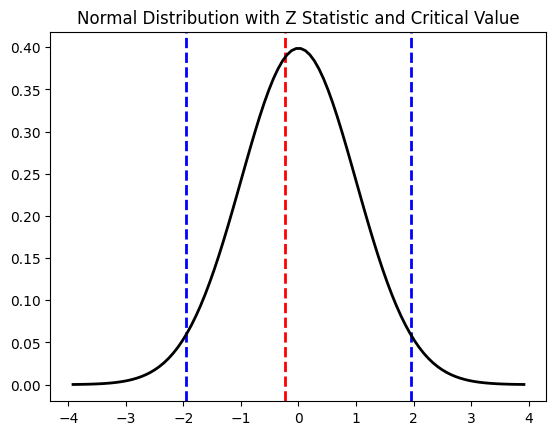
\includegraphics[width=0.8\textwidth]{images/result_1.png}
    \caption{Resultado de la prueba de hipótesis de diferencia de medias, se muestra el intevalo crítico (azul), junto al resultado del estadístico de prueba (rojo).}
\end{figure}

Finalmente, se repitió el proceso en el segundo caso, un modelo con tres servidores vs un modelo con uno solo el triple de rápido:

\begin{figure}[H]
   \centering
   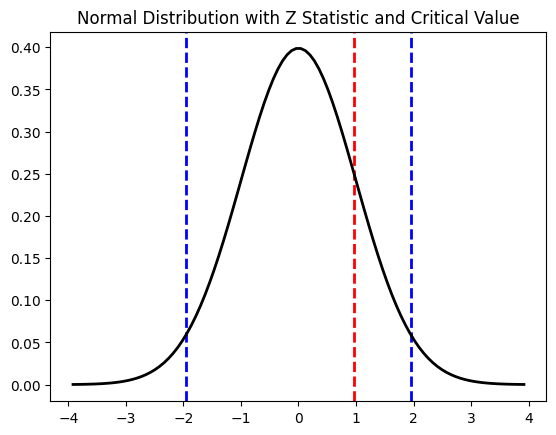
\includegraphics[width=0.8\textwidth]{images/result_2.png}
    \caption{Resultado de la prueba de hipótesis de diferencia de medias, se muestra el intevalo crítico (azul), junto al resultado del estadístico de prueba (rojo).}
\end{figure}

De esta forma, no podemos rechazar la hipótesis de que no existan diferencias significativas entre los modelos, lo cual es un resultado interesante.

El flujo de trabajo que está en la notebook facilita la repetción de estos experimentos, para diferentes combinaciones de modelos.

\end{document}

